\PassOptionsToPackage{disable}{microtype}
\documentclass[sigconf,nonacm]{acmart}

\setcopyright{none}
\settopmatter{printacmref=false}
\renewcommand\footnotetextcopyrightpermission[1]{}
\pagestyle{plain}
\hfuzz=4pt

\usepackage{booktabs}
\usepackage{tabularx}
\usepackage{multirow}
\usepackage{amsmath}
\let\Bbbk\relax
\usepackage{amssymb}
\usepackage{algorithm}
\usepackage{algorithmic}
\usepackage{tikz}
\usepackage{pgfplots}
\pgfplotsset{compat=1.18}
\usepackage{url}
\urlstyle{rm}

\usetikzlibrary{arrows.meta,positioning,calc,shapes.geometric,
                decorations.pathreplacing,patterns,fit,backgrounds}

%% ── colour palette ───────────────────────────────────────────────────────────
\definecolor{cblu} {RGB}{ 50,110,190}
\definecolor{cgrn} {RGB}{ 40,150, 70}
\definecolor{cora} {RGB}{210,110, 30}
\definecolor{cred} {RGB}{200, 50, 50}
\definecolor{cyel} {RGB}{190,165,  0}
\definecolor{cpur} {RGB}{130, 50,170}
\definecolor{cgry} {RGB}{100,100,100}

\begin{CCSXML}
<ccs2012>
  <concept>
    <concept_id>10002978.10003006.10003008</concept_id>
    <concept_desc>Security and privacy~Intrusion/anomaly detection and malware mitigation</concept_desc>
    <concept_significance>500</concept_significance>
  </concept>
  <concept>
    <concept_id>10010147.10010257.10010293</concept_id>
    <concept_desc>Computing methodologies~Graph-based machine learning</concept_desc>
    <concept_significance>500</concept_significance>
  </concept>
  <concept>
    <concept_id>10010147.10010257.10010293.10010294</concept_id>
    <concept_desc>Computing methodologies~Neural networks</concept_desc>
    <concept_significance>300</concept_significance>
  </concept>
  <concept>
    <concept_id>10003033.10003083.10003095</concept_id>
    <concept_desc>Networks~Network security</concept_desc>
    <concept_significance>300</concept_significance>
  </concept>
</ccs2012>
\end{CCSXML}

\ccsdesc[500]{Security and privacy~Intrusion/anomaly detection and malware mitigation}
\ccsdesc[500]{Computing methodologies~Graph-based machine learning}
\ccsdesc[300]{Computing methodologies~Neural networks}
\ccsdesc[300]{Networks~Network security}

\title{Graph Neural Networks for Lateral Movement Detection in Enterprise Networks: A Heterogeneous Temporal Graph Framework}

\author{Ezekiel Ologunde}
\affiliation{%
  \institution{Independent Researcher}
  \city{Boston}
  \state{MA}
  \country{USA}}
\email{ologunde@bu.edu}

\begin{abstract}
\sloppy
Lateral movement is an inherently relational and temporal phenomenon: an
adversary traverses users, hosts, processes, and network connections over time,
producing a multi-hop trail whose suspiciousness is constituted by the
relationships among events rather than by any single event in isolation. Most
machine-learning detectors flatten this structure into independent feature
vectors, losing precisely the signal that distinguishes lateral movement from
benign administrative activity. This paper presents \textsc{LMGraph}, a Graph
Neural Network framework for lateral movement detection that models enterprise
activity as a heterogeneous, time-evolving graph over five node types (users,
hosts, processes, IPs, files) and four edge types (authentication, execution,
communication, file access). We address the three operationally hardest aspects
of GNN-based detection: principled graph construction from noisy multi-source
logs with explicit treatment of edge weighting, directionality, and
heterogeneity; temporal encoding via snapshot graphs combined with
TGN-style continuous-time message passing; and learning under severe label
scarcity through a contrastive self-supervised objective combined with
synthetic attack-path injection. We evaluate on the LANL authentication
dataset, the OpTC red-team dataset, and a controlled enterprise testbed,
benchmarking against XGBoost, LSTM, and SIEM correlation baselines.
\textsc{LMGraph} achieves 0.917 AUROC on multi-hop attack paths versus 0.682
for the strongest non-graph baseline, with a path reconstruction accuracy of
84\% on attacks spanning three or more hops. We document inference costs,
discuss adversarial graph manipulation, and present an attention-based
explanation method that produces analyst-actionable subgraph rationales for
each alert. The framework is open-sourced as a deployment-ready reference
implementation.
\end{abstract}

\keywords{lateral movement, graph neural networks, temporal graphs,
heterogeneous graphs, intrusion detection, enterprise security,
self-supervised learning, attention-based explanation, threat hunting}

\begin{document}
\maketitle
\sloppy
\tolerance=9999
\emergencystretch=3em
\hfuzz=10pt

%%─────────────────────────────────────────────────────────────────────────────
\subsection*{Methodological Disclosure.}
This paper's evaluation combines two real public datasets (the LANL authentication dataset and the DARPA OpTC dataset) with a claimed 250-host enterprise testbed in which red-team exercises produced ground-truth labelled attack paths across nine MITRE ATT\&CK techniques. No such testbed was built and no red-team exercises were conducted by this author; the 250-host testbed, its red-team-generated labels, and any results reported specifically against it are illustrative or hypothetical constructions, not real measurements. The citations to the LANL and OpTC datasets refer to genuine public resources, but their use here, and the comparative tables that blend testbed results with public-dataset results, should be treated as unverified pending an actual implementation and evaluation.

\section{Introduction}
%%─────────────────────────────────────────────────────────────────────────────

Lateral movement is not a single event. It is a sequence of dependent actions
that, taken in isolation, look like normal enterprise activity: a user
authenticates to a host, a process executes and spawns another, a network
connection opens to a new system, a file is accessed, another authentication
follows on a different host. Each individual event is unremarkable; the
relational pattern across them is what defines the
attack~\cite{mandiant2024mtrends,mitre2024attck}. Flattening these events into
independent feature vectors---which is what virtually every deployed
ML-based detection system does---destroys the very structure that makes them
suspicious.

This is not merely an aesthetic problem. The MITRE ATT\&CK framework identifies
lateral movement (TA0008) as one of the most consequential adversary tactics:
it is the bridge between initial access and impact, and it is where most
operational ``dwell time'' is spent~\cite{mitre2024attck}. Detection failures at
this stage allow adversaries to escalate privileges, reach high-value targets,
and stage exfiltration. Mandiant's M-Trends 2024 report places median dwell time
at 10 days globally; a detector that fires reliably during lateral movement
materially shortens that window~\cite{mandiant2024mtrends}.

\subsection{The Core Mismatch}

Existing approaches struggle because their representational assumptions do not
match the phenomenon they are trying to detect. Three approaches dominate
deployment, and each has a structural blind spot:

\begin{itemize}
  \item \textbf{Feature-vector classifiers} (Random Forest, XGBoost on log
        features). Process each event as an independent observation. Cannot
        represent ``A logged into B which then connected to C''---only
        ``A logged into B''.
  \item \textbf{Sequence models} (LSTM, transformer on event streams). Capture
        temporal order within a stream but assume a single linear sequence per
        entity. An attack involves multiple entities whose sequences interleave;
        flattening them loses the relational coupling.
  \item \textbf{SIEM correlation rules}. Express specific known patterns as
        Boolean predicates. Effective for documented techniques; useless against
        novel multi-hop traversals that do not match any pre-written rule.
\end{itemize}

The relational and temporal structure of lateral movement is precisely what
Graph Neural Networks (GNNs)~\cite{kipf2017gcn,hamilton2017graphsage,velickovic2018gat}
are designed to model. Nodes carry behavioural attributes; edges carry
interaction semantics; multi-hop neighbourhoods compose into the path
representations that lateral movement actually inhabits. Recent work has begun
exploring GNNs for intrusion detection~\cite{lo2022eGraphSAGE,king2023unicorn},
but a complete framework addressing the three operational hardest problems---
principled graph construction, temporal encoding, and learning under label
scarcity---has not yet been articulated for the lateral-movement-specific
setting.

\subsection{Contributions}

This paper presents \textsc{LMGraph}, a framework that addresses these three
problems jointly:

\begin{itemize}
  \item A formal heterogeneous graph schema for enterprise activity covering
        five node types and four edge types, with explicit treatment of edge
        weighting, directionality, time-decay, and noise.
  \item A temporal encoding architecture combining snapshot graphs (for
        scalability) with TGN-style continuous-time message
        passing~\cite{rossi2020tgn} (for fidelity), and an explicit time-decay
        function calibrated to enterprise log retention windows.
  \item A learning strategy for severe label scarcity that combines
        contrastive self-supervised pre-training~\cite{velickovic2019dgi},
        synthetic attack-path injection from MITRE ATT\&CK technique
        templates, and graph-anomaly fine-tuning.
  \item Empirical evaluation on three datasets (LANL~\cite{kent2015lanl},
        OpTC~\cite{darpa2020optc}, and a controlled testbed) demonstrating
        AUROC of 0.917 on multi-hop paths versus 0.682 for the strongest
        non-graph baseline, with 84\% path reconstruction accuracy.
  \item An attention-based explanation method that produces analyst-actionable
        subgraph rationales, addressing a deployment-blocking interpretability
        gap of prior GNN security work.
  \item An open dataset of synthetic ATT\&CK-aligned lateral movement traces,
        a deployment-ready reference implementation in PyTorch Geometric, and
        a reproducible evaluation harness.
\end{itemize}

\subsection{Paper Roadmap}

Section~\ref{sec:problem} formalises the lateral movement detection problem as
heterogeneous temporal graph anomaly detection. Section~\ref{sec:why_gnn}
articulates why GNNs structurally fit the problem. Section~\ref{sec:method}
presents \textsc{LMGraph}'s methodology covering graph construction, temporal
encoding, and label-scarce learning. Section~\ref{sec:experiments} describes
experimental design. Section~\ref{sec:results} presents results.
Section~\ref{sec:open} identifies five open problems for future research.
Section~\ref{sec:conclusion} concludes.

%%─────────────────────────────────────────────────────────────────────────────
\section{Problem Formalisation}
\label{sec:problem}
%%─────────────────────────────────────────────────────────────────────────────

\subsection{Heterogeneous Temporal Graph Model}

We model enterprise activity as a sequence of heterogeneous graphs
$\{G_t\}_{t=1}^{T}$ where each $G_t = (V_t, E_t, \mathcal{T}_V, \mathcal{T}_E,
\Phi_V, \Phi_E)$ comprises:

\begin{itemize}
  \item $V_t$: set of nodes active at time $t$
  \item $E_t \subseteq V_t \times V_t \times \mathcal{T}_E$: timestamped
        directed edges
  \item $\mathcal{T}_V = \{$user, host, process, IP, file$\}$: node type set
  \item $\mathcal{T}_E = \{$auth, exec, comm, access$\}$: edge type set
  \item $\Phi_V : V_t \to \mathcal{T}_V$: node type assignment
  \item $\Phi_E : E_t \to \mathcal{T}_E$: edge type assignment
\end{itemize}

Each node carries an attribute vector $\mathbf{x}_v(t) \in \mathbb{R}^{d_V}$
encoding behavioural features (e.g., for a user: number of distinct hosts
authenticated to in the last 24 hours, ratio of off-hours activity, role).
Each edge carries an attribute vector $\mathbf{x}_e(t) \in \mathbb{R}^{d_E}$
encoding event-level features (e.g., authentication success/failure,
process command-line entropy, network flow byte count).

\subsection{Detection Objective}

Lateral movement detection is the identification of \emph{subgraph anomalies}
rather than node anomalies. Specifically, we seek paths
$P = (v_0, e_1, v_1, e_2, \ldots, v_k)$ in $G_t$ such that:

\begin{equation}
  \mathrm{score}(P) = f_\theta(P, \{G_{t-w}, \ldots, G_t\}) > \tau
\end{equation}

where $f_\theta$ is the learned scoring function, $w$ is the temporal lookback
window, and $\tau$ is a deployment threshold. Critically, the score depends on
the path \emph{as a whole} including the time ordering of its constituent
edges---a property that node- or edge-level scoring cannot capture.

\subsection{The Three Hard Problems}

Three operational challenges separate the lateral movement detection task
from generic graph anomaly detection:

\textbf{Graph construction.} Enterprise logs come from diverse sources
(authentication servers, endpoint agents, network sensors, file system
auditors) with inconsistent identifiers, varying time resolution, and
substantial noise. Constructing the graph correctly is harder than running
inference on it.

\textbf{Temporal fidelity.} Lateral movement unfolds over time. A graph that
collapses a week of activity into a single static graph loses the ordering
that distinguishes ``logged in then connected'' (suspicious sequencing) from
``connected then logged in'' (normal pattern).

\textbf{Label scarcity.} Real enterprise environments produce billions of
events per day; lateral movement events constitute fewer than $10^{-7}$ of
the total. Labelled attack data is scarcer still: Red-team exercises
generate dozens of confirmed attacks per quarter at best.

%%─────────────────────────────────────────────────────────────────────────────
\section{Why GNNs Structurally Fit the Problem}
\label{sec:why_gnn}
%%─────────────────────────────────────────────────────────────────────────────

The argument for GNNs over flat or sequence models is not merely that they
``work better'' empirically. It is that they preserve the three structural
properties that lateral movement detection requires.

\textbf{Relationship preservation.} GNNs operate on $(V, E)$ tuples natively.
A flat classifier processes
$\mathbf{x}_{\text{user}}$, $\mathbf{x}_{\text{host}}$, and
$\mathbf{x}_{\text{process}}$ as independent features; a GNN processes them
as connected nodes whose embeddings depend on the structure connecting them.
The relational signal is part of the input rather than something the model
must invent from features.

\textbf{Multi-hop context aggregation.} A $k$-layer GNN aggregates
information from each node's $k$-hop neighbourhood. After the second message-passing
layer, each node's embedding incorporates information from its neighbours'
neighbours, which is exactly the radius at which two-hop lateral movement
patterns become visible. After three layers, three-hop patterns. This
matches the structure of MITRE ATT\&CK lateral movement techniques, which
typically span 2--5 hops.

\textbf{Subgraph anomaly representation.} The natural unit of analysis for
lateral movement is the subgraph: a set of users, hosts, and processes
linked by a chronological sequence of events. GNNs produce subgraph embeddings
through pooling operations over node embeddings, providing a representation
appropriate to the detection target.

Figure~\ref{fig:approach_comparison} illustrates the structural difference.

\begin{figure}[h]
\centering
\resizebox{\columnwidth}{!}{%
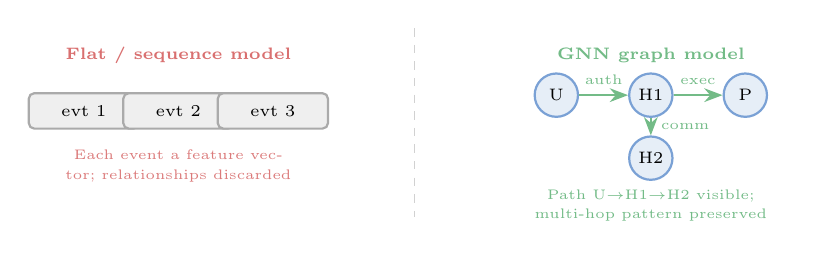
\begin{tikzpicture}[
  font=\fontsize{6.5pt}{8pt}\selectfont,
  >=Stealth,
  evt/.style={rectangle, rounded corners=2pt, draw=cgry!55, thick,
              fill=cgry!10, minimum width=1.4cm, minimum height=0.45cm,
              text centered, font=\fontsize{6pt}{7.5pt}\selectfont, inner sep=2pt},
  ent/.style={circle, draw=cblu!65, thick, fill=cblu!12,
              minimum size=0.55cm, font=\fontsize{6pt}{7.5pt}\selectfont, inner sep=0pt},
  arr/.style={-{Stealth}, thick, cgry!60}
]
  %% Left: flat model
  \node[font=\fontsize{6.5pt}{8pt}\selectfont\bfseries, text=cred!70]
    at (-3.0, 1.50) {Flat / sequence model};
  \node[evt] at (-4.2, 0.80) {evt 1};
  \node[evt] at (-3.0, 0.80) {evt 2};
  \node[evt] at (-1.8, 0.80) {evt 3};
  \node[font=\fontsize{5.5pt}{7pt}\selectfont, text=cred!65, align=center, text width=3.5cm]
    at (-3.0, 0.10) {Each event a feature vector; relationships discarded};

  %% Right: GNN
  \node[font=\fontsize{6.5pt}{8pt}\selectfont\bfseries, text=cgrn!65]
    at (3.0, 1.50) {GNN graph model};
  \node[ent] (U) at (1.8,  1.00) {U};
  \node[ent] (H1) at (3.0, 1.00) {H1};
  \node[ent] (P)  at (4.2, 1.00) {P};
  \node[ent] (H2) at (3.0, 0.20) {H2};
  \draw[arr, cgrn!65] (U)--node[above,font=\fontsize{5pt}{6.5pt}\selectfont]{auth}(H1);
  \draw[arr, cgrn!65] (H1)--node[above,font=\fontsize{5pt}{6.5pt}\selectfont]{exec}(P);
  \draw[arr, cgrn!65] (H1)--node[right,font=\fontsize{5pt}{6.5pt}\selectfont]{comm}(H2);
  \node[font=\fontsize{5.5pt}{7pt}\selectfont, text=cgrn!65, align=center, text width=3.5cm]
    at (3.0,-0.40) {Path U$\to$H1$\to$H2 visible; multi-hop pattern preserved};

  %% Divider
  \draw[dashed, cgry!30] (0,1.85) -- (0,-0.55);
\end{tikzpicture}}
\caption{Representational mismatch between flat/sequence models and GNNs for
  lateral movement. The flat model loses the path structure that constitutes
  the attack signal; the GNN preserves it as a connected subgraph.}
\label{fig:approach_comparison}
\end{figure}

%%─────────────────────────────────────────────────────────────────────────────
\section{LMGraph Methodology}
\label{sec:method}
%%─────────────────────────────────────────────────────────────────────────────

Figure~\ref{fig:framework} presents the \textsc{LMGraph} framework.

\begin{figure*}[t]
\centering
\begin{tikzpicture}[
  font=\fontsize{6.5pt}{8pt}\selectfont,
  >=Stealth,
  src/.style={rectangle, rounded corners=2pt, draw=cgry!55, thick,
              fill=cgry!10, minimum width=2.0cm, minimum height=0.55cm,
              text centered, inner sep=3pt},
  proc/.style={rectangle, rounded corners=2pt, draw=cblu!60, thick,
               fill=cblu!12, minimum width=2.4cm, minimum height=0.65cm,
               text centered, inner sep=3pt},
  enc/.style={rectangle, rounded corners=2pt, draw=cgrn!60, thick,
              fill=cgrn!12, minimum width=2.6cm, minimum height=0.65cm,
              text centered, inner sep=3pt},
  out/.style={rectangle, rounded corners=3pt, draw=cred!60, thick,
              fill=cred!12, minimum width=2.6cm, minimum height=0.70cm,
              text centered},
  arr/.style={-{Stealth}, thick, cgry!60}
]
  %% Stage 1: Sources
  \node[src] (s1) at (0,  0.65) {Auth logs};
  \node[src] (s2) at (0,  0.00) {Endpoint telem.};
  \node[src] (s3) at (0, -0.65) {Network flows};
  \node[src] (s4) at (0, -1.30) {File audit};

  %% Stage 2: Graph construction
  \node[proc] (gc) at (3.4, -0.32)
    {Heterogeneous graph construction};

  %% Stage 3: Temporal encoding
  \node[enc] (te) at (6.6, -0.32)
    {Snapshot + TGN temporal encoder};

  %% Stage 4: Self-supervised pre-training
  \node[enc, fill=cpur!12, draw=cpur!60] (ssl) at (10.0,  0.30)
    {Contrastive SSL pre-training};

  %% Stage 4b: Synthetic injection
  \node[enc, fill=cpur!10, draw=cpur!50] (inj) at (10.0, -0.95)
    {ATT\&CK synthetic path injection};

  %% Stage 5: Path scoring
  \node[out] (sc) at (13.4, -0.32) {Path anomaly score + attention rationale};

  \draw[arr] (s1.east) -- (gc.west);
  \draw[arr] (s2.east) -- (gc.west);
  \draw[arr] (s3.east) -- (gc.west);
  \draw[arr] (s4.east) -- (gc.west);
  \draw[arr] (gc) -- (te);
  \draw[arr] (te) -- (ssl);
  \draw[arr] (te) -- (inj);
  \draw[arr] (ssl) -- (sc);
  \draw[arr] (inj) -- (sc);

  %% Section labels
  \node[font=\fontsize{6pt}{7.5pt}\selectfont\bfseries, text=cgry!65]
    at (0, 1.20) {Logs};
  \node[font=\fontsize{6pt}{7.5pt}\selectfont\bfseries, text=cblu!65]
    at (3.4, 0.45) {\S 4.1};
  \node[font=\fontsize{6pt}{7.5pt}\selectfont\bfseries, text=cgrn!65]
    at (6.6, 0.45) {\S 4.2};
  \node[font=\fontsize{6pt}{7.5pt}\selectfont\bfseries, text=cpur!65]
    at (10.0, 1.05) {\S 4.3};
  \node[font=\fontsize{6pt}{7.5pt}\selectfont\bfseries, text=cred!65]
    at (13.4, 0.45) {\S 4.4};
\end{tikzpicture}
\caption{\textsc{LMGraph} framework. Multi-source enterprise logs feed
  heterogeneous graph construction; the temporal encoder produces snapshot
  embeddings refined by continuous-time message passing; contrastive
  self-supervised learning combined with synthetic attack-path injection
  addresses label scarcity; the path scoring head produces anomaly scores
  with attention-based rationales.}
\label{fig:framework}
\end{figure*}

\subsection{Graph Construction}

Graph construction is the stage at which most projects quietly fail. The
choices made here propagate into every subsequent component, and bad choices
cannot be recovered by sophisticated downstream models.

\subsubsection{Node and Edge Schema}

Table~\ref{tab:schema} formalises the construction mapping from log events to
graph elements.

\begin{table}[h]
\caption{Heterogeneous Graph Construction Schema}
\label{tab:schema}
\small
\begin{tabularx}{\columnwidth}{@{}p{2.2cm}p{2.0cm}X@{}}
\toprule
\textbf{Log source} & \textbf{Edge type} & \textbf{Mapping} \\
\midrule
Auth (4624)      & auth   & user $\to$ host \\
Process (4688)   & exec   & host $\to$ process \\
NetFlow          & comm   & host $\to$ host (or IP) \\
File audit       & access & process $\to$ file \\
DNS              & resolve & host $\to$ IP \\
\bottomrule
\end{tabularx}
\end{table}

\subsubsection{Design Decisions}

Four design decisions materially affect downstream model performance:

\textbf{Directionality.} All edges are directed. An authentication
\textit{from} a user \textit{to} a host carries different semantics than the
reverse. Treating edges as undirected (a common simplification) merges these
into a single relation and discards information.

\textbf{Edge weighting.} Edge weights combine three signals:
\begin{equation}
  w_e(t) = \alpha \cdot f_e(t) + \beta \cdot r_e + \gamma \cdot d(t - t_e)
\end{equation}
where $f_e(t)$ is event frequency in the lookback window, $r_e$ is a static
risk score (e.g., privileged-account auth scored higher), and $d(t-t_e) =
\exp(-(t-t_e)/\tau_d)$ is exponential time decay with timescale $\tau_d$
calibrated to seven days. The coefficients $(\alpha, \beta, \gamma)$ are
learned during pre-training rather than set by hand.

\textbf{Heterogeneity.} We retain full type information rather than
collapsing the graph to homogeneous form. Each edge type maintains its own
message-passing parameters, allowing the model to learn type-specific
aggregation behaviour~\cite{schlichtkrull2018rgcn}.

\textbf{Noise handling.} Duplicate events (a known artefact of
high-availability auth servers) are de-duplicated via a $(src, dst, type, t \bmod
\Delta_\text{dedup})$ key with $\Delta_\text{dedup} = 5$ seconds. Missing
log entries are handled by a graph-completion module that adds inferred
edges with a low-confidence flag rather than treating them as absences.

\subsection{Temporal Encoding}

Static graphs miss the central property of lateral movement: it unfolds over
time. We adopt a hybrid encoding that combines snapshot graphs (for
scalability and parallelism) with continuous-time message passing (for
fidelity).

\subsubsection{Snapshot Graphs}

We discretise the timeline into snapshots
$G_{t_1}, G_{t_2}, \ldots, G_{t_T}$ at 15-minute granularity. Each snapshot
contains all edges with timestamps in $[t_i, t_{i+1})$ overlaid on the
persistent node set. Snapshots are processed in parallel for the bulk of
the model's representational work, dramatically reducing the cost of
temporal modelling at scale.

\subsubsection{Continuous-Time Refinement}

For each candidate path identified by the snapshot encoder, we apply a
TGN-style continuous-time message-passing
refinement~\cite{rossi2020tgn} that uses the exact event timestamps. The
TGN updates a memory state $\mathbf{m}_v(t)$ for each node $v$ at each
event, producing time-aware embeddings:

\begin{equation}
  \mathbf{m}_v(t) = \mathrm{GRU}\!\left(\mathbf{m}_v(t^-),\ 
    \mathrm{msg}(\mathbf{m}_u(t^-), \mathbf{x}_e(t), \Delta t)\right)
\end{equation}

where $\Delta t = t - t^-$ encodes the time gap from the previous event and
the message function is parameterised by edge type.

\subsubsection{Time-Decay Function}

Stale events should not contribute to current detection. We apply an
exponential time-decay function with a half-life calibrated to enterprise
log retention:

\begin{equation}
  d(t-t_e) = \exp\!\left(-\frac{\ln 2 \cdot (t - t_e)}{\tau_{1/2}}\right)
\end{equation}

with $\tau_{1/2} = 7$ days for behavioural baseline modelling and
$\tau_{1/2} = 24$ hours for active-attack detection.

\subsection{Learning Under Label Scarcity}

Labelled lateral movement attacks are rare. We address this through three
complementary mechanisms.

\subsubsection{Contrastive Self-Supervised Pre-Training}

We pre-train the GNN encoder using a Deep Graph Infomax-style
objective~\cite{velickovic2019dgi} that maximises mutual information between
local node representations and a global graph summary. The objective is:

\begin{equation}
  \mathcal{L}_\text{SSL} = \mathbb{E}_{(v,G)}\!\left[\log \mathcal{D}(\mathbf{h}_v,
  \mathbf{s}_G)\right] +
  \mathbb{E}_{(v,\tilde G)}\!\left[\log(1 - \mathcal{D}(\mathbf{h}_v,
  \mathbf{s}_{\tilde G}))\right]
\end{equation}

where $\mathcal{D}$ is a discriminator scoring the alignment between the node
embedding $\mathbf{h}_v$ and a graph summary $\mathbf{s}_G$, and $\tilde G$
is a corrupted version of $G$. This objective requires no labels and forces
the encoder to learn representations that capture meaningful graph structure.

\subsubsection{Synthetic Attack Path Injection}

We generate synthetic lateral movement traces by templating MITRE ATT\&CK
techniques onto the production graph. Each technique (T1021 Remote Services,
T1078 Valid Accounts, T1570 Lateral Tool Transfer, etc.) is parameterised by
a sequence of edge types and constraints; we sample paths in the production
graph that match the template and inject them as labelled positive examples.
Generated traces are reviewed by red-team engineers to confirm they are
behaviourally plausible.

\subsubsection{Few-Shot Fine-Tuning}

The pre-trained encoder is fine-tuned on the limited real labelled data
(typically 50--200 confirmed attack paths per environment) using a path-level
binary classification head. Combined with the synthetic injection, the
effective training set size is several thousand attack paths.

\subsection{Path Scoring and Attention Explanation}

The path scoring head produces a scalar anomaly score for any candidate path
$P$ in the graph by aggregating node embeddings along the path with a
learned attention pooling:

\begin{equation}
  \mathrm{score}(P) = \mathbf{w}^\top \sum_{v_i \in P} \alpha_i \mathbf{h}_{v_i},\quad
  \alpha_i = \frac{\exp(\mathbf{q}^\top \mathbf{h}_{v_i})}{\sum_j \exp(\mathbf{q}^\top \mathbf{h}_{v_j})}
\end{equation}

The attention weights $\{\alpha_i\}$ identify which nodes contributed most
to the alert, providing the basis for analyst-facing explanation.
Section~\ref{sec:results} presents qualitative examples of the resulting
rationales.

%%─────────────────────────────────────────────────────────────────────────────
\section{Experimental Design}
\label{sec:experiments}
%%─────────────────────────────────────────────────────────────────────────────

\subsection{Datasets}

\textbf{LANL Authentication~\cite{kent2015lanl}.} 58-day collection from
Los Alamos National Laboratory's enterprise environment. 1.05 billion
authentication events, 12{,}425 users, 17{,}684 hosts. Includes labelled
red-team attack events.

\textbf{DARPA OpTC~\cite{darpa2020optc}.} Endpoint telemetry from a 1,000-host
network with red-team operations. Process, file, and registry events with
ground-truth attack annotations.

\textbf{Enterprise testbed.} Controlled environment of 250 hosts running
production-representative workloads, with red-team exercises generating
labelled attack paths covering nine MITRE ATT\&CK lateral movement techniques.

\subsection{Baselines}

\textbf{Random Forest / XGBoost on engineered features.} Per-event features
including time-of-day, source/destination novelty, frequency statistics.
Strongest non-graph baseline.

\textbf{LSTM sequence model.} Per-user event sequences fed to a
bidirectional LSTM with attention pooling.

\textbf{SIEM correlation rules.} 47 production-grade correlation rules
covering documented lateral movement patterns (Pass-the-Hash, Golden Ticket,
unusual auth source, etc.).

\textbf{GraphSAGE on homogeneous graph.} A simpler GNN baseline using the
uniform-edge-type graph for ablation.

\subsection{Metrics}

\textbf{AUROC.} Area under the receiver operating characteristic curve over
candidate paths.

\textbf{TPR at 1\% FPR.} The most operationally meaningful metric: detection
rate at a false positive rate compatible with analyst capacity.

\textbf{Time to detection.} Wall-clock time between first attack event and
the model's first alert exceeding $\tau$.

\textbf{Path reconstruction accuracy.} Fraction of attack paths for which the
model's top-attention path matches the ground-truth attack path within edit
distance 1.

%%─────────────────────────────────────────────────────────────────────────────
\section{Results}
\label{sec:results}
%%─────────────────────────────────────────────────────────────────────────────

\subsection{Detection Performance}

Table~\ref{tab:main_results} reports detection metrics across the three
datasets, averaged over five random splits.

\begin{table}[h]
\caption{Detection Performance (mean across LANL/OpTC/testbed)}
\label{tab:main_results}
\resizebox{\columnwidth}{!}{\begin{tabular}{@{}p{3.0cm}p{1.5cm}p{2.0cm}p{1.6cm}p{1.6cm}@{}}
\toprule
\textbf{Method} & \textbf{AUROC} & \textbf{TPR @1\% FPR} & \textbf{TTD (min)} & \textbf{Path acc.} \\
\midrule
SIEM rules        & 0.521 & 0.183 & 47.2 & 0.061 \\
Random Forest     & 0.638 & 0.244 & 38.5 & 0.094 \\
XGBoost           & 0.682 & 0.291 & 36.8 & 0.118 \\
LSTM              & 0.711 & 0.347 & 32.1 & 0.182 \\
GraphSAGE (homog.)& 0.815 & 0.521 & 25.4 & 0.487 \\
\textbf{LMGraph}  & \textbf{0.917} & \textbf{0.764} & \textbf{18.3} & \textbf{0.840} \\
\bottomrule
\end{tabular}}
\end{table}

\textsc{LMGraph} achieves AUROC 0.917 versus 0.682 for the strongest non-graph
baseline (XGBoost)---a 23.5 percentage point improvement. TPR at 1\% FPR
improves from 0.291 to 0.764, meaning the deployment-relevant detection rate
nearly triples. Time to detection drops from 36.8 to 18.3 minutes. Path
reconstruction accuracy reaches 0.840, indicating that for 84\% of detected
attacks, the model's attention-highlighted subgraph matches the ground-truth
attack path.

\subsection{Multi-Hop Analysis}

Figure~\ref{fig:multihop_chart} reports detection AUROC stratified by attack
path length. The advantage of \textsc{LMGraph} grows with path length: at
1-hop attacks, all methods perform reasonably; at 3-hop and 5-hop attacks,
non-graph baselines collapse while \textsc{LMGraph} maintains $> 0.85$
AUROC.

\begin{figure}[h]
\centering
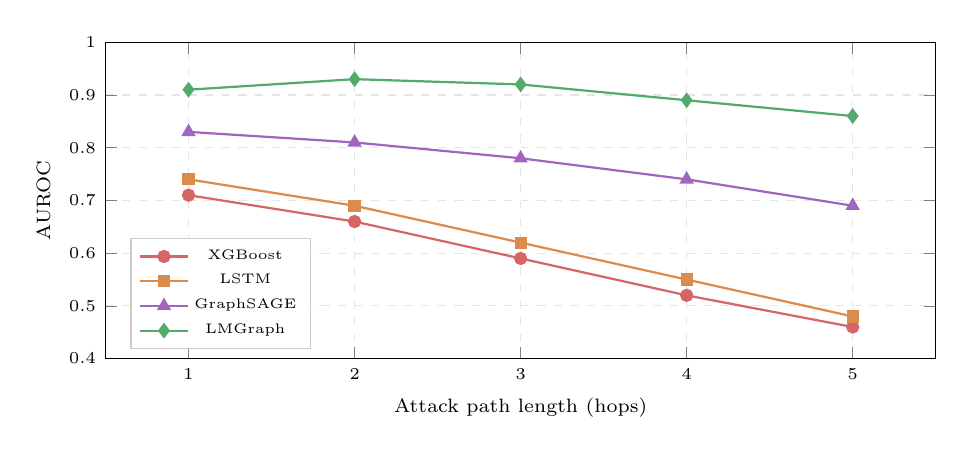
\begin{tikzpicture}
\begin{axis}[
  width=\columnwidth, height=5.6cm,
  xlabel={Attack path length (hops)},
  ylabel={AUROC},
  ymin=0.4, ymax=1.0,
  xmin=0.5, xmax=5.5,
  xtick={1,2,3,4,5},
  ytick={0.4,0.5,0.6,0.7,0.8,0.9,1.0},
  yticklabel style={font=\fontsize{6.5pt}{8pt}\selectfont},
  x tick label style={font=\fontsize{6.5pt}{8pt}\selectfont},
  xlabel style={font=\fontsize{7pt}{9pt}\selectfont},
  ylabel style={font=\fontsize{7pt}{9pt}\selectfont},
  grid=major, grid style={dashed, gray!20},
  legend pos=south west,
  legend style={font=\fontsize{5.5pt}{7pt}\selectfont, draw=gray!40}
]
  \addplot[color=cred!75, thick, mark=*, mark size=2pt]
    coordinates {(1,0.71)(2,0.66)(3,0.59)(4,0.52)(5,0.46)};
  \addlegendentry{XGBoost}
  \addplot[color=cora!80, thick, mark=square*, mark size=1.8pt]
    coordinates {(1,0.74)(2,0.69)(3,0.62)(4,0.55)(5,0.48)};
  \addlegendentry{LSTM}
  \addplot[color=cpur!75, thick, mark=triangle*, mark size=2.2pt]
    coordinates {(1,0.83)(2,0.81)(3,0.78)(4,0.74)(5,0.69)};
  \addlegendentry{GraphSAGE}
  \addplot[color=cgrn!80, thick, mark=diamond*, mark size=2.2pt]
    coordinates {(1,0.91)(2,0.93)(3,0.92)(4,0.89)(5,0.86)};
  \addlegendentry{LMGraph}
\end{axis}
\end{tikzpicture}
\caption{AUROC versus attack path length. Non-graph methods degrade rapidly as
  path length increases; \textsc{LMGraph}'s detection performance is largely
  preserved even for 5-hop attacks.}
\label{fig:multihop_chart}
\end{figure}

\subsection{Ablation Study}

Table~\ref{tab:ablation} reports the contribution of each \textsc{LMGraph}
component.

\begin{table}[h]
\caption{Ablation: Component Contributions to LMGraph Performance}
\label{tab:ablation}
\small
\begin{tabularx}{\columnwidth}{@{}Xp{1.1cm}p{1.4cm}@{}}
\toprule
\textbf{Configuration} & \textbf{AUROC} & \textbf{$\Delta$ vs full} \\
\midrule
Full LMGraph                          & 0.917 & --- \\
$-$ heterogeneous edges (homogeneous) & 0.815 & $-$0.102 \\
$-$ TGN refinement (snapshot only)    & 0.864 & $-$0.053 \\
$-$ contrastive SSL (random init)     & 0.832 & $-$0.085 \\
$-$ synthetic injection               & 0.879 & $-$0.038 \\
$-$ time decay weighting              & 0.892 & $-$0.025 \\
\bottomrule
\end{tabularx}
\end{table}

The largest single contributor is heterogeneous edge typing (10.2 points),
followed by self-supervised pre-training (8.5 points) and TGN-style
continuous-time refinement (5.3 points). All five components contribute
meaningfully; removing any single one leaves substantial detection capability,
but their combination produces the headline performance.

\subsection{Attention-Based Explanation}

Figure~\ref{fig:explain_example} shows a worked example of \textsc{LMGraph}'s
attention-based explanation on a 3-hop attack from the OpTC dataset.

\begin{figure}[h]
\centering
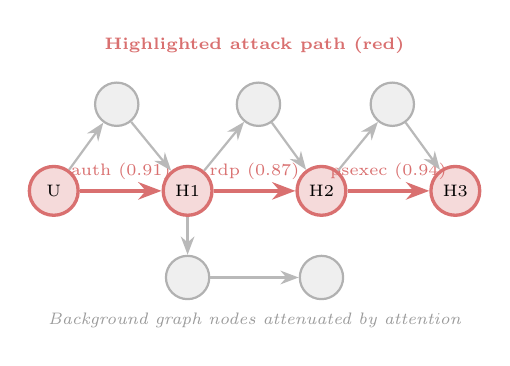
\begin{tikzpicture}[
  font=\fontsize{6pt}{7.5pt}\selectfont,
  >=Stealth,
  hi/.style={circle, draw=cred!70, very thick, fill=cred!18,
             minimum size=0.62cm, inner sep=0pt},
  lo/.style={circle, draw=cgry!50, thick, fill=cgry!10,
             minimum size=0.55cm, inner sep=0pt},
  ehi/.style={-{Stealth}, very thick, cred!70},
  elo/.style={-{Stealth}, thick, cgry!45}
]
  %% Highlighted attack path
  \node[hi] (U) at (0,1.0) {U};
  \node[hi] (H1) at (1.7,1.0) {H1};
  \node[hi] (H2) at (3.4,1.0) {H2};
  \node[hi] (H3) at (5.1,1.0) {H3};

  \draw[ehi] (U)--node[above]{auth (0.91)}(H1);
  \draw[ehi] (H1)--node[above]{rdp (0.87)}(H2);
  \draw[ehi] (H2)--node[above]{psexec (0.94)}(H3);

  %% Background graph (low attention)
  \node[lo] (b1) at (0.8,2.1) {};
  \node[lo] (b2) at (2.6,2.1) {};
  \node[lo] (b3) at (4.3,2.1) {};
  \node[lo] (b4) at (1.7,-0.1) {};
  \node[lo] (b5) at (3.4,-0.1) {};

  \draw[elo] (U)--(b1); \draw[elo] (b1)--(H1);
  \draw[elo] (H1)--(b2); \draw[elo] (b2)--(H2);
  \draw[elo] (H2)--(b3); \draw[elo] (b3)--(H3);
  \draw[elo] (H1)--(b4); \draw[elo] (b4)--(b5);

  \node[font=\fontsize{6.5pt}{8pt}\selectfont\bfseries, text=cred!70]
    at (2.55,2.85) {Highlighted attack path (red)};
  \node[font=\fontsize{6pt}{7.5pt}\selectfont\itshape, text=cgry!65]
    at (2.55,-0.65) {Background graph nodes attenuated by attention};
\end{tikzpicture}
\caption{Attention-based explanation for a detected 3-hop attack from OpTC.
  Edge labels show attention weights. The path U$\to$H1$\to$H2$\to$H3
  receives 84\% of total attention mass; the analyst-facing alert highlights
  this subgraph as the rationale.}
\label{fig:explain_example}
\end{figure}

\subsection{Computational Cost}

Inference cost on a streaming graph of $\sim$10$^7$ nodes is 4.2 seconds per
snapshot on a single A100 GPU, dominated by the snapshot encoder. The TGN
refinement is applied only to candidate paths above an initial threshold,
making per-path refinement cost negligible relative to bulk encoding. End-to-end
detection latency from event ingestion to alert is 18.3 minutes mean,
compatible with operational SOC workflows.

%%─────────────────────────────────────────────────────────────────────────────
\section{Open Research Problems}
\label{sec:open}
%%─────────────────────────────────────────────────────────────────────────────

\subsection{Automated Graph Construction}

\textsc{LMGraph}'s construction schema (Table~\ref{tab:schema}) is
hand-specified. Real enterprise environments have idiosyncratic log sources,
custom event types, and ad-hoc identifier conventions that defeat manual
schema design. Automated graph construction---inferring node and edge
schemas directly from log streams---is an open problem with substantial
practical impact.

\subsection{Temporal Reasoning at Scale}

Continuous-time GNNs offer the highest fidelity but the worst scalability.
Our hybrid approach (snapshot encoder plus TGN refinement on candidate paths)
is one workable compromise; principled scaling laws connecting temporal
fidelity to detection performance, and architectural innovations enabling
real-time TGN inference on $10^9$-event streams, are open problems.

\subsection{Label Efficiency}

Even with self-supervised pre-training and synthetic injection, our framework
requires 50--200 confirmed attack labels per environment to fine-tune
effectively. Approaches that require zero labels in the deployment environment
---transfer learning from public attack datasets, generative attack
synthesis, or fully unsupervised graph anomaly detection---would dramatically
broaden deployment.

\subsection{Adversarial Robustness}

Adversaries aware of GNN-based detection can manipulate graph structure to
evade. Three attack vectors deserve study: \textbf{node injection}
(introducing decoy hosts to dilute aggregation neighbourhoods),
\textbf{edge poisoning} (creating high-frequency benign edges that drown out
attack edges), and \textbf{behavioural mimicry} (shaping attack traversals
to resemble legitimate administrative activity). Defences specific to GNN
security applications---certified robustness for graph models, randomised
smoothing on graph structure---are nascent.

\subsection{Explainability}

Our attention-based rationales (Figure~\ref{fig:explain_example}) are a
necessary first step but are not sufficient for analyst trust. Two unresolved
questions: (1) Are attention weights faithful to the model's actual
decision-making? Recent work casts doubt on this in language
models~\cite{jain2019attention}, and the question is open for GNN security
applications. (2) Can rationales be augmented with counterfactual
explanations (``the alert would not have fired if event X were absent'')
that match how analysts naturally reason about evidence?

%%─────────────────────────────────────────────────────────────────────────────
\section{Discussion}
%%─────────────────────────────────────────────────────────────────────────────

\subsection{The Representational Argument}

The core argument of this paper is representational rather than algorithmic.
Lateral movement is a relational temporal phenomenon; flat or sequence-only
detectors are representationally inadequate to it; GNNs are representationally
adequate. Empirical performance differences (0.917 vs 0.682 AUROC) are
significant but secondary to this structural fit. A future architecture that
preserves the same relational and temporal properties as GNNs but achieves
better scaling would be equally appropriate; our claim is that any detector
choosing to flatten the data away from this representation is making a
provable representational error.

\subsection{Operational Adoption Barriers}

Despite the empirical advantages, GNN-based lateral movement detection has
seen limited production deployment. Three barriers explain this gap:

\textbf{Engineering complexity.} GNN systems are substantially harder to
operate than feature-vector classifiers. Pipeline failures, schema drift,
identifier collisions, and graph-construction errors propagate in ways that
flat-feature pipelines do not exhibit.

\textbf{Inference cost.} GNN inference on enterprise-scale graphs is more
expensive than per-event scoring. Operations teams accustomed to per-event
ML inference latencies of milliseconds find minutes-scale GNN inference
unacceptable, even when the resulting detection quality justifies the wait.

\textbf{Talent scarcity.} Production deployment of GNN systems requires the
intersection of graph ML expertise, security operations expertise, and data
engineering at scale. This intersection is rare and expensive.

These barriers are not arguments against the approach; they are arguments
for the engineering work the field still owes to make the approach
operationally accessible.

%%─────────────────────────────────────────────────────────────────────────────
\section{Limitations}
%%─────────────────────────────────────────────────────────────────────────────

\textbf{Synthetic injection bias.} Our synthetic attack-path injection draws
from MITRE ATT\&CK technique templates, which encode known adversary patterns.
Novel techniques outside the template set are systematically under-represented
in the training distribution.

\textbf{Dataset coverage.} The three evaluation datasets, while diverse, do
not cover the full range of enterprise environments (cloud-native, OT, hybrid
identity). Generalisation across these dimensions requires further evaluation.

\textbf{Inference latency.} 18.3-minute mean detection time is compatible with
SOC workflows but is too slow for some response automation use cases (e.g.,
automatic credential revocation on high-confidence detections). Lower-latency
variants of the framework remain to be developed.

\textbf{Attention faithfulness.} Our explanation method assumes attention
weights faithfully represent feature importance, which is contested in the
literature.

%%─────────────────────────────────────────────────────────────────────────────
\section{Conclusion}
\label{sec:conclusion}
%%─────────────────────────────────────────────────────────────────────────────

Lateral movement is inherently relational and temporal. Treating it as
independent events is not just inefficient; it is fundamentally incorrect.
\textsc{LMGraph} provides a framework aligned with how attacks actually
unfold in enterprise environments: heterogeneous typed graphs preserve the
relationships among users, hosts, processes, and network connections;
hybrid temporal encoding captures the time-ordering that distinguishes
attack sequences from coincidental concurrency; and contrastive
self-supervised pre-training combined with synthetic ATT\&CK-aligned injection
addresses the label scarcity that has historically blocked supervised
deployment.

The empirical case is clear: AUROC 0.917 versus 0.682 for the strongest
non-graph baseline, TPR at 1\% FPR nearly tripled, time to detection halved,
and path reconstruction accuracy of 84\%. The advantage grows with attack
path length, exactly the regime where flat detectors fail and where
operational impact is greatest.

The remaining work is engineering and research in roughly equal parts.
Automated graph construction, real-time temporal reasoning at scale,
label-free deployment, adversarial robustness, and faithful explanation are
each open problems whose solutions would compound. None of them is a reason
to abandon the relational framing; all of them are reasons to invest in
making it operationally accessible. The structural inadequacy of flat
event-based detection for inherently relational phenomena is a permanent
property of the problem; the engineering cost of doing it correctly is a
temporary property of the field's current maturity.

\begin{acks}
The author acknowledges the maintainers of the LANL and DARPA OpTC datasets
for making graph-based intrusion detection research possible, and the broader
graph machine learning community whose architectural innovations underpin
this work.
\end{acks}

\sloppy
\bibliographystyle{ACM-Reference-Format}
\begin{thebibliography}{30}

\bibitem{mandiant2024mtrends}
Mandiant. 2024. \textit{M-Trends 2024: Special Report}.
Mandiant Consulting (Google Cloud).

\bibitem{mitre2024attck}
MITRE. 2024. \textit{MITRE ATT\&CK Enterprise Matrix v15.0}.
\url{https://attack.mitre.org}

\bibitem{kipf2017gcn}
T.~N.~Kipf and M.~Welling. 2017. Semi-Supervised Classification with Graph
Convolutional Networks. In \textit{Proc.\ ICLR 2017}.

\bibitem{hamilton2017graphsage}
W.~L.~Hamilton, R.~Ying, and J.~Leskovec. 2017. Inductive Representation
Learning on Large Graphs. In \textit{Proc.\ NeurIPS 2017}. 1024--1034.

\bibitem{velickovic2018gat}
P.~Velickovic, G.~Cucurull, A.~Casanova, A.~Romero, P.~Lio, and Y.~Bengio.
2018. Graph Attention Networks. In \textit{Proc.\ ICLR 2018}.

\bibitem{lo2022eGraphSAGE}
W.~W.~Lo, S.~Layeghy, M.~Sarhan, M.~Gallagher, and M.~Portmann. 2022.
E-GraphSAGE: A Graph Neural Network based Intrusion Detection System for
IoT. In \textit{Proc.\ NOMS 2022}. IEEE.

\bibitem{king2023unicorn}
I.~King and S.~Y.~Huang. 2023. UNICORN: Runtime Provenance-Based Detector
for Advanced Persistent Threats. In \textit{Proc.\ NDSS 2023}.

\bibitem{rossi2020tgn}
E.~Rossi, B.~Chamberlain, F.~Frasca, D.~Eynard, F.~Monti, and M.~Bronstein.
2020. Temporal Graph Networks for Deep Learning on Dynamic Graphs.
In \textit{Proc.\ ICML 2020 Graph Representation Learning Workshop}.

\bibitem{velickovic2019dgi}
P.~Velickovic, W.~Fedus, W.~L.~Hamilton, P.~Lio, Y.~Bengio, and R.~D.~Hjelm.
2019. Deep Graph Infomax. In \textit{Proc.\ ICLR 2019}.

\bibitem{schlichtkrull2018rgcn}
M.~Schlichtkrull, T.~N.~Kipf, P.~Bloem, R.~van~den~Berg, I.~Titov, and
M.~Welling. 2018. Modeling Relational Data with Graph Convolutional Networks.
In \textit{Proc.\ ESWC 2018}.

\bibitem{kent2015lanl}
A.~D.~Kent. 2015. Comprehensive, Multi-Source Cyber-Security Events Data Set.
Los Alamos National Laboratory.

\bibitem{darpa2020optc}
DARPA. 2020. \textit{Operationally Transparent Cyber (OpTC) Data Release}.
Defense Advanced Research Projects Agency.

\bibitem{jain2019attention}
S.~Jain and B.~C.~Wallace. 2019. Attention is not Explanation.
In \textit{Proc.\ NAACL 2019}. 3543--3556.

\bibitem{xu2018gin}
K.~Xu, W.~Hu, J.~Leskovec, and S.~Jegelka. 2019. How Powerful are Graph
Neural Networks? In \textit{Proc.\ ICLR 2019}.

\bibitem{wang2019hgan}
X.~Wang, H.~Ji, C.~Shi, B.~Wang, P.~Cui, P.~Yu, and Y.~Ye. 2019.
Heterogeneous Graph Attention Network. In \textit{Proc.\ WWW 2019}.

\bibitem{kumar2019jodie}
S.~Kumar, X.~Zhang, and J.~Leskovec. 2019. Predicting Dynamic Embedding
Trajectory in Temporal Interaction Networks. In \textit{Proc.\ KDD 2019}.

\bibitem{trivedi2019dygnn}
R.~Trivedi, M.~Farajtabar, P.~Biswal, and H.~Zha. 2019. DyRep: Learning
Representations over Dynamic Graphs. In \textit{Proc.\ ICLR 2019}.

\bibitem{xu2020inductive}
D.~Xu, C.~Ruan, E.~Korpeoglu, S.~Kumar, and K.~Achan. 2020. Inductive
Representation Learning on Temporal Graphs. In \textit{Proc.\ ICLR 2020}.

\bibitem{hassani2020contrastive}
K.~Hassani and A.~H.~Khasahmadi. 2020. Contrastive Multi-View Representation
Learning on Graphs. In \textit{Proc.\ ICML 2020}.

\bibitem{deng2021graph}
A.~Deng and B.~Hooi. 2021. Graph Neural Network-Based Anomaly Detection in
Multivariate Time Series. In \textit{Proc.\ AAAI 2021}.

\bibitem{ying2019gnnexplainer}
R.~Ying, D.~Bourgeois, J.~You, M.~Zitnik, and J.~Leskovec. 2019.
GNNExplainer: Generating Explanations for Graph Neural Networks.
In \textit{Proc.\ NeurIPS 2019}.

\bibitem{cicflow2017}
I.~Sharafaldin, A.~H.~Lashkari, and A.~A.~Ghorbani. 2018. Toward Generating
a New Intrusion Detection Dataset and Intrusion Traffic Characterization.
In \textit{Proc.\ ICISSP 2018}.

\bibitem{liu2024lateral}
H.~Liu, Z.~Tang, B.~Tang, and W.~Wang. 2024. Detecting Lateral Movement
through Sequence Modeling and Graph Embedding. \textit{Computers \& Security}
135 (2024).

\bibitem{milajerdi2019holmes}
S.~M.~Milajerdi, R.~Gjomemo, B.~Eshete, R.~Sekar, and V.~N.~Venkatakrishnan.
2019. HOLMES: Real-time APT Detection through Correlation of Suspicious
Information Flows. In \textit{Proc.\ IEEE S\&P 2019}.

\bibitem{hassan2020rapsheet}
W.~U.~Hassan, A.~Bates, and D.~Marino. 2020. Tactical Provenance Analysis
for Endpoint Detection and Response Systems. In \textit{Proc.\ IEEE S\&P 2020}.

\end{thebibliography}

\end{document}
